\documentclass{article}
\usepackage[utf8]{inputenc}
\usepackage{amssymb}
\usepackage{amsfonts}
\usepackage{graphicx} %package to manage images
\usepackage{multirow}
\usepackage[table,xcdraw]{xcolor}
\usepackage{amsmath}
\usepackage{booktabs}
\usepackage{caption}
\usepackage{comment}
\usepackage{floatrow}
\floatstyle{plaintop}
\restylefloat{table}
\title{Appendix}
\begin{document}
\section*{\hfil Appendix \hfil}

This appendix provides the supplementary research material including detailed descriptions of data and menu generation artificial intelligence.

\section{Menu generation artificial intelligence}
\subsection{Data}
In this work, we used food and diet data. Food data include the nutrients and ingredients of 1,726 foods and consist of 20 nutrition columns and 298 ingredient columns. Table \ref{table: table1} shows a sample row of the food data.

\begin{table}[ht]
\begin{tabular}{|c|c|c|c|c|c|}
\hline
\textbf{Food}   & \textbf{Energy(kcal)} & \textbf{Carbohydrate(g)} & ... & \textbf{Cabbage} & \textbf{Pumpkin} \\ \hline
Kimchi & 6.250  & 1.100        & ... & 1       & 0       \\ \hline
\end{tabular}
\caption{Sample row of the foods dataset}
\label{table: table1}
\end{table}

Food data consist of the nutrition, ingredients, and group information. The nutrition part shows the nutrients in a standard serving of each food. The ingredients information signifies whether the specific food contains a specific ingredient. For example, kimchi contains cabbage but not pumpkin, so the cabbage column is indicated as 1, and the pumpkin column is indicated as 0. The group information indicates the type of food such as soup, main dish, and side dish. In this dataset, foods are grouped according to the list of dishes in Korean cuisine.

The diet dataset comprises a standard diet from one of the government Centers for Children’s Food Service Management Korea. This center was established by the Ministry of Food and Drug Safety to support hygiene and nutrition management for daycare centers and kindergartens. The diet provided in this dataset was designed by professional nutritionists and disclosed to the public. These data are used as a reference for planning diets in kindergartens. Each row is a collection of food items, and the entire dataset consisted of 220 rows consumed from February to November 2019 (excluding weekends and holidays). Table \ref{table: table2} shows a sample of the diet dataset. As shown in Table \ref{table: table2}, the 1st and 2nd cells are morning snacks, the 3rd to 7th are lunch, the 8th and 9th are afternoon snacks, and the 10th to 14th are dinner, representing the standard daily diet of a Korean nursery and does not include breakfast.\footnote{Due to the lack of space, we illustrate our sample as multiple rows in Table \ref{table: table2}. However, the real sample in our dataset is unfolded into one row.} Each diet plan is described in order of main dish-soup-side dish. Not all 14 cells are always filled, some are empty for diet plans consisting of fewer kinds of nutritionally complete foods.


\begin{table}[ht]
\caption{Sample row of the foods dataset}
\begin{tabular}{|c|c|c|c|c|c|}
\hline
\textbf{Date}           & \multicolumn{5}{c|}{\textbf{Menu}}                                                                                                                                                        \\ \hline
\multirow{8}{*}{July 2} & \textbf{morning 1}   & \textbf{morning 2}   & \textbf{}                                                    & \textbf{}                                                &                   \\ \cline{2-6} 
                        & Carrot stick         & milk                 &                                                              &                                                          &                   \\ \cline{2-6} 
                        & \textbf{lunch 1}     & \textbf{lunch 2}     & \textbf{lunch 3}                                             & \textbf{lunch 4}                                         & \textbf{lunch 5}  \\ \cline{2-6} 
                        & Jjajangbap           & Miso soup            & Dumplings                                                    & Kimchi                                                   & (empty)           \\ \cline{2-6} 
                        & \textbf{afternoon 1} & \textbf{afternoon 2} & \textbf{}                                                    & \textbf{}                                                &                   \\ \cline{2-6} 
                        & White Bread          & Yogurt               &                                                              &                                                          &                   \\ \cline{2-6} 
                        & \textbf{dinner 1}    & \textbf{dinner 2}    & \textbf{dinner 3}                                            & \textbf{dinner 4}                                        & \textbf{dinner 5} \\ \cline{2-6} 
                        & White Rice           & Fish cake soup       & \begin{tabular}[c]{@{}c@{}}Boiled pork\\ slices\end{tabular} & \begin{tabular}[c]{@{}c@{}}Cucumber\\ salad\end{tabular} & Kimchi            \\ \hline
\end{tabular}
\label{table: table2}
\end{table}

\subsection{Artificial Intelligence}
In this section, we describe the methods that underlie the two AI solutions of Generative Adversarial Nets and Reinforcement Learning.

\subsubsection{Generative Adversarial Nets}
Generative Adversarial Nets (GAN) is a framework for training the generator model through its competition with the discriminator model. In GAN, the generator model (G) and the discriminator model (D) are initially trained with real data. The purpose of G is to estimate the real data distribution, and the purpose of D is to distinguish between real and generated data. G generates data that mimic the real data based on the estimated data distribution, and D returns the probability that inputted data were derived from real data. Therefore, the purpose of G is to ensure that D recognizes the data generated by G as real data (not generated). It is proven that the output of D converges to 0.5 when G and D are ideal (i.e., when G and D are well-trained)\cite{goodfellow2014generative}.\footnote{D has nothing but tossing a coin to judge whether the inputted data is real or not as G succeeds to perfectly deceive D.}

\begin{figure}[ht]
    \centering
    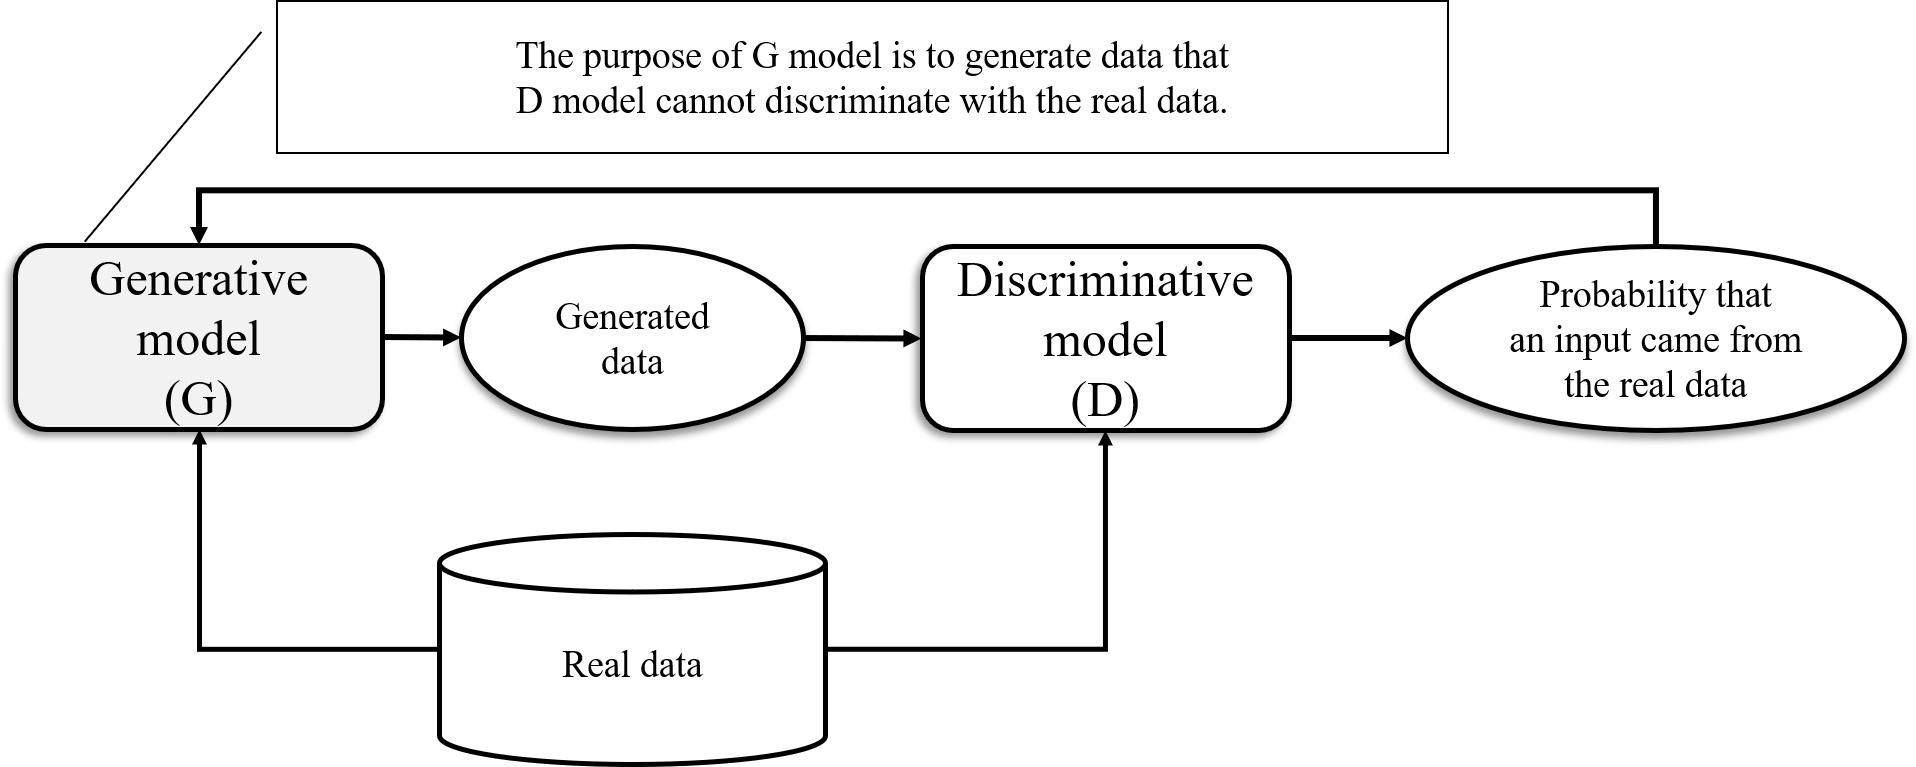
\includegraphics[width = 12cm, height = 4.81cm]{images/GAN_framework.png}
    \caption{The framework of Generative Adversarial Nets}
    \label{fig:GAN_Framework}
\end{figure} 

Entering each food directly into the GAN is not effective. Because GAN uses only real data and only 752 have been used in real data among 1,726 foods, then the generated diet will consist of only these 752 items of food. To utilize all the 1,726 foods, we categorized foods and transformed the diet data from the level of individual food to the level of food category. This way, foods that were not used in the daily diet data can appear in the generated diet if other foods in the same category have been used. 
First, we categorized the foods that make up the diet using the Affinity propagation clustering algorithm \cite{frey2007clustering}. Each set of foods produced through this categorization is called a food cluster, and each cluster is numbered. 
Categorization was based on the ingredients that make up the food and created 154 clusters. For example, a list of foods belonging to Cluster 6 includes dried-shrimp potato stew, dried-shrimp chard stew, dried-shrimp miso stew, dried-shrimp consommé, dried-shrimp daikon stew, and tofu stew. We can see that most of Cluster 6 consists of stews with dried shrimp. After categorization, we replaced each food in the diet data with the index number of the relevant cluster. For example, dried-shrimp potato stew belongs to Cluster 6, so this dish is replaced by a ’6’. Finally, we encode the clusters of diet data into binary format of their relevant foods. The cell where the food item (row) belongs to the cluster number (column) is indicated by a ‘1,’ and the remaining cells are zeros.
Figure 2 shows an example of this transformation process, changing diet data into the data that can be used for GAN. We used GAN to train a diet-generating model with the real data.

\begin{figure}[!ht]
    \centering
    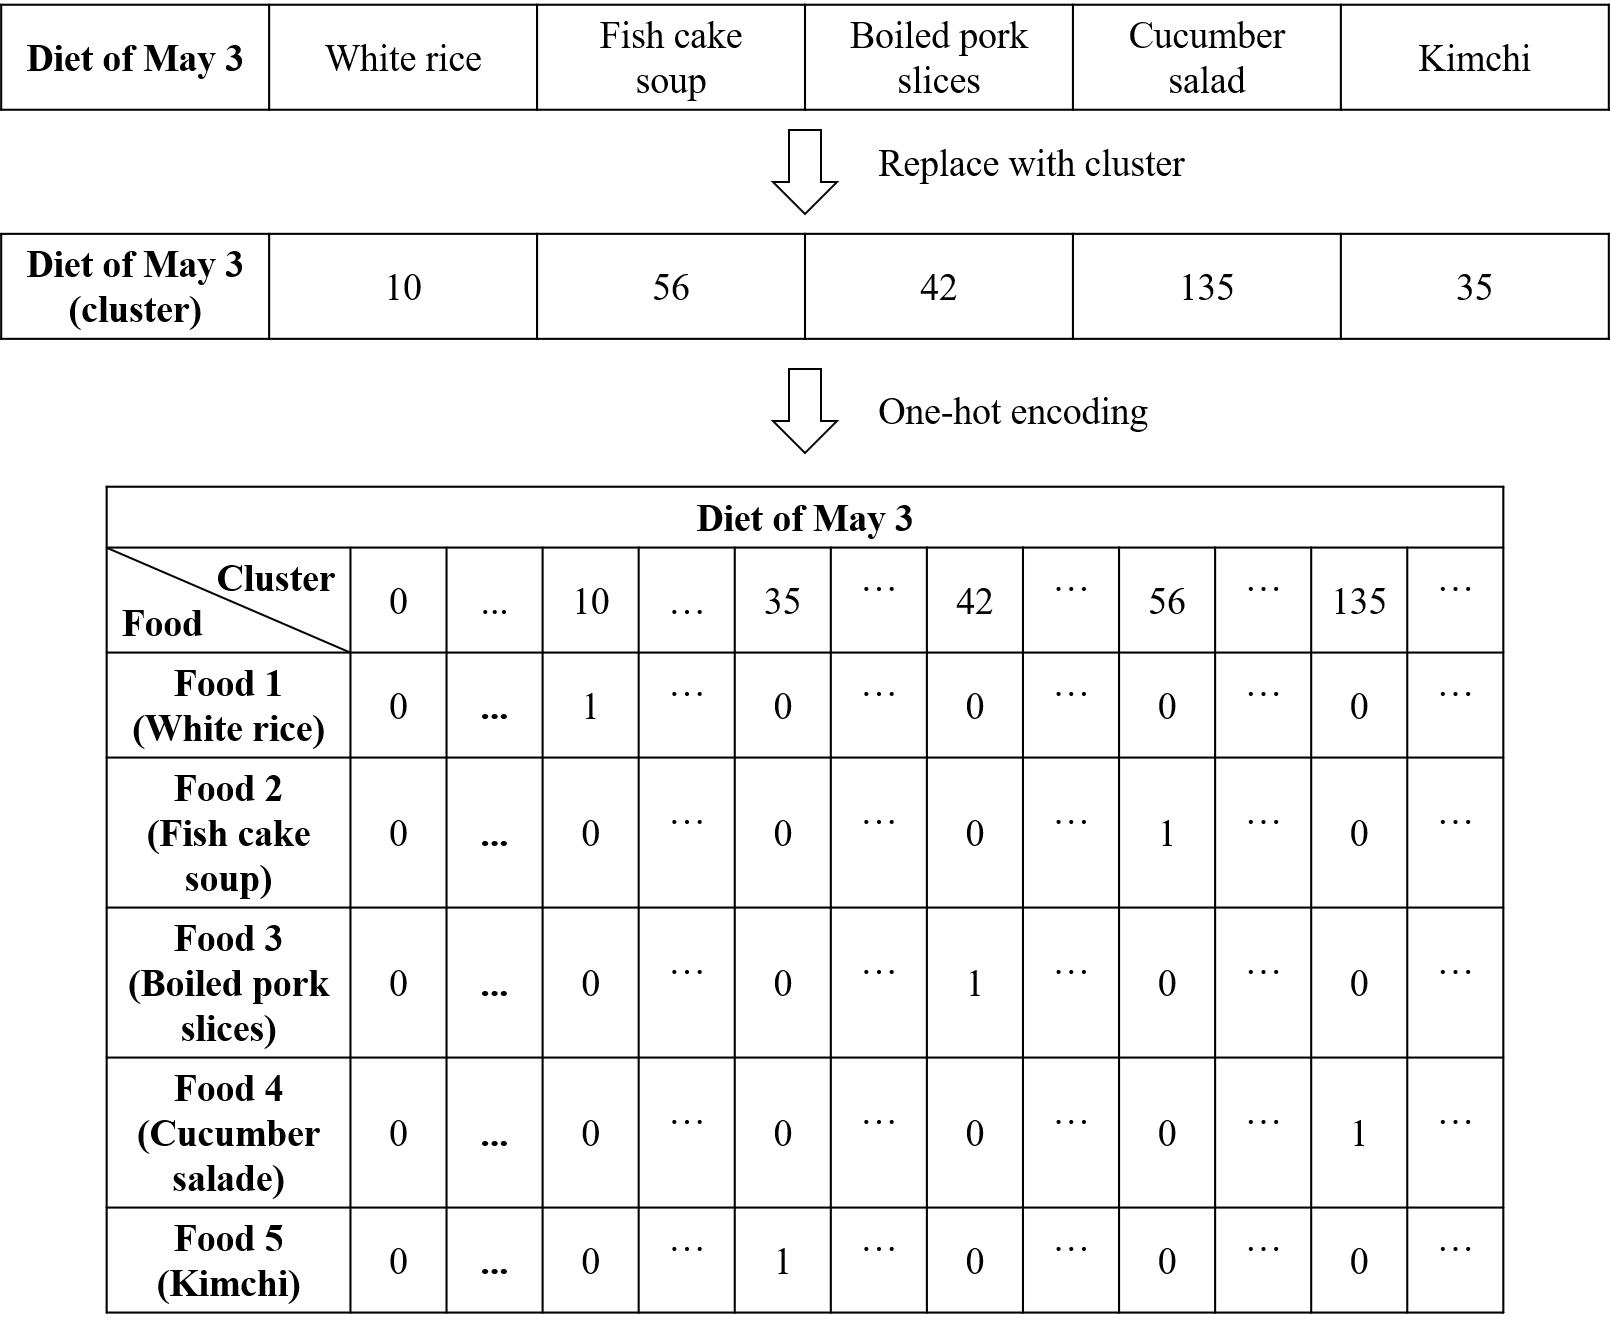
\includegraphics[width = 11cm, height = 8.62cm]{images/menu_transform.png}
    \caption{Data transformation process from food to cluster}
    \label{fig:GAN_transform}
\end{figure} 

The generator model learned through the GAN process generates diets of food clusters in the form shown in Table \ref{table: table2}. We should revert these cluster-level results back to original food-level form. For this, we return the encoded data to cluster number data through a reverse of the transformation process described earlier. Then, each cell is replaced with a randomly selected food in the relevant cluster. Figure 3 shows an example of this restoration process.

\begin{figure}[!ht]
    \centering
    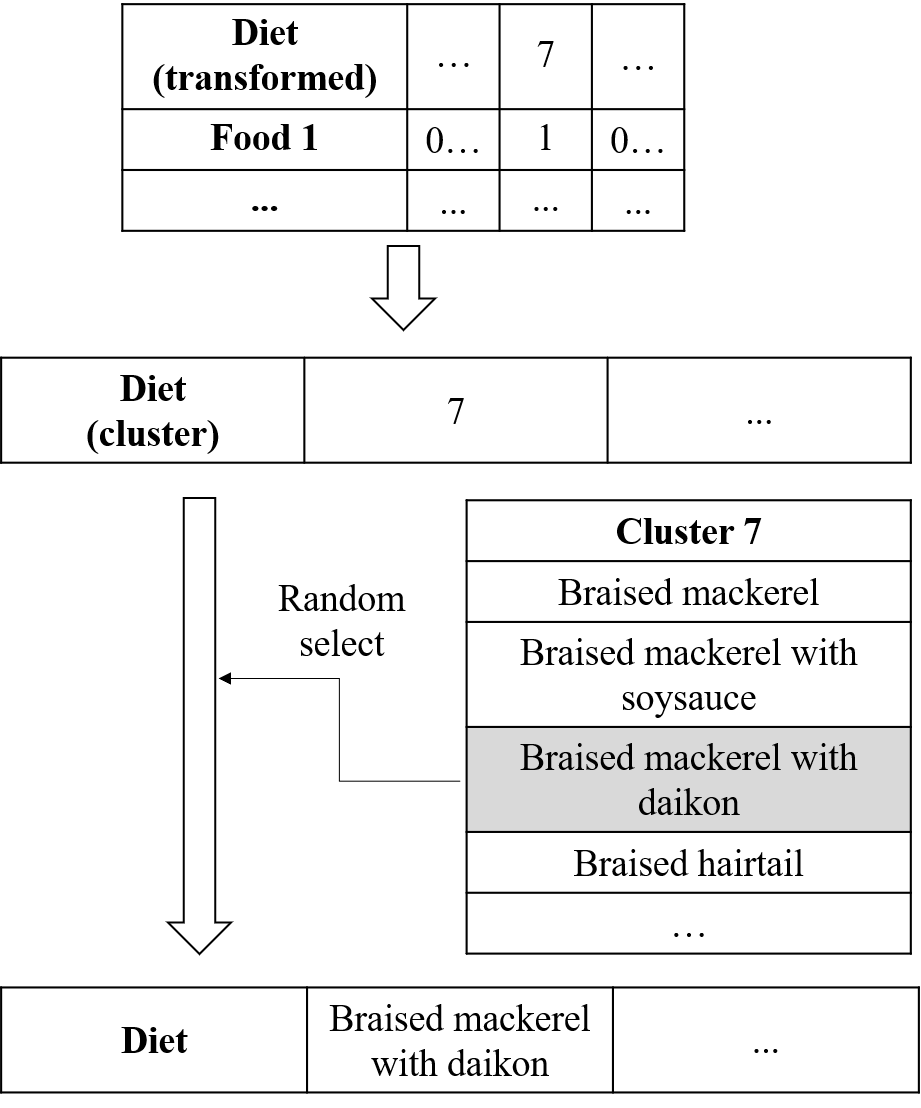
\includegraphics[width = 6cm, height = 7.6cm]{images/menu_restore.png}
    \caption{Data restoration process from cluster to food}
    \label{fig:GAN_restore}
\end{figure} 

%We carried out classifications three times on different criteria: nutrition, ingredients and nutrition & ingredients. Therefore, each food belongs to three clusters each formed by different criteria. For example, bulgogi belongs to cluster 92 in the nutrient-based classification, cluster 121 in the ingredients-based classification and cluster 91 in the nutrition & ingredients-based classification. 116 clusters were created in the nutrient-based classification, 158 in the ingredients-based classification and 161 in the nutrition & ingredients-based classification.

\newpage
\subsubsection{Reinforcement Learning (RL)} 

Reinforcement learning (RL) evolved out of efforts to model animal behavior such as mice trying to find their way through a maze to a reward \cite{powell2020}. RL aims to develop an agent to learn the behavior (i.e., policy) that reinforces the correct decision (i.e., action) through a framework of trial-and-error interactions in a dynamic environment \cite{kaelbling1996reinforcement} (See Figure \ref{fig:Framework}). RL is a principled mathematical framework, where an agent learns correct decisions by experiencing consecutive situations and optimizes her sequential decisions. As a result, for the past few years RL has arisen as one of the most promising method in AI research that studies sequential decision-making over time.

\begin{figure}[ht]
    \centering
    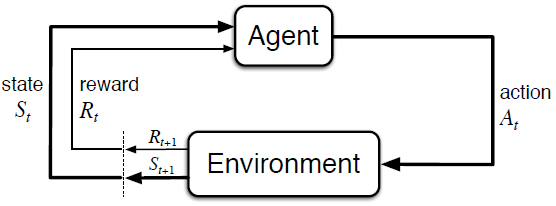
\includegraphics[width = 10cm, height = 3.5cm]{images/RL_Framework.PNG}
    \caption{The agent - environment interaction in reinforcement learning \cite{sutton1998introduction}}
    \label{fig:Framework}
\end{figure}

The task of RL is usually described as a Markov Decision Process (MDP), a class of stochastic sequential decision processes in which each decision only depends on the previous decisions and their outcomes \cite{sutton1998introduction, puterman1990markov}. A MDP consists of:

\begin{itemize}
    \item a set of states $\mathcal{S}$
    \item a set of actions $\mathcal{A}$
    \item a reward function $\mathbb{R}: \mathcal{S} \times \mathcal{A} \rightarrow \mathcal{R}$
    \item a discount factor $\gamma$
    \item a transition function $\mathbb{T}: \mathcal{S} \times \mathcal{A} \rightarrow \mathcal{P}$ 
\end{itemize}

\noindent where $\mathcal{S}$ is a set of observable states, and each state is an agent's observation of a situation. $\mathcal{A}$ is a set of feasible actions from which the agent selects to act. The agent behaves differently according to the current state. How an agent will behave depends on the policy $\pi$, which is the parameterized probability distribution of actions and defines the probability that an agent will select each action at the given state.

$\mathbb{R}$ is a reward function that maps the given state and action onto a reward, which is the only information that the agent learns from the environment. Equation \ref{eq:Reward function} shows the numerical expression of reward function that is defined as the expected value of the reward. Given that the state is $\mathnormal{S}_{t} = \mathnormal{s}$ and the action is $\mathnormal{A}_{t} = \mathnormal{a}$ at time $\mathnormal{t}$, the agent receives a reward according to the reward function.

\begin{equation}
    r(s_{t}, a_{t}) = \mathbb{E}[R_{t+1}|S_{t} = s, A_{t} = a] = R_{t+1}
\label{eq:Reward function}
\end{equation}

The agent makes a decision (i.e., selects an action) as follows. In an MDP setting, successive decisions are made over time. Therefore, the agent needs to consider the future situation caused by the current decision. To do this, a discount factor $\gamma$ is introduced. Total return to the agent at time $t$ is determined as follows:

\begin{equation}
    G_{t} = R_{t+1} + \gamma R_{t+2} + \gamma^{2} R_{t+3} + \gamma^{3} R_{t+4} + ...
    \label{eq:Gain}
\end{equation}

The environment provides not only a reward to the agent, but also a next state, as determined by the transition function $\mathbb{T}$. The transition function defines $P_{s, a}^{s'}$, the probability of states that the environment will return as a next state $\mathnormal{S}_{t+1} = s'$ when the agent takes action $\mathnormal{A}_{t} = a$ at the given state $\mathnormal{S}_{t} = s$. Because the environment underlies the transition function, it is called an environment model. 

\begin{figure}[ht]
    \centering
    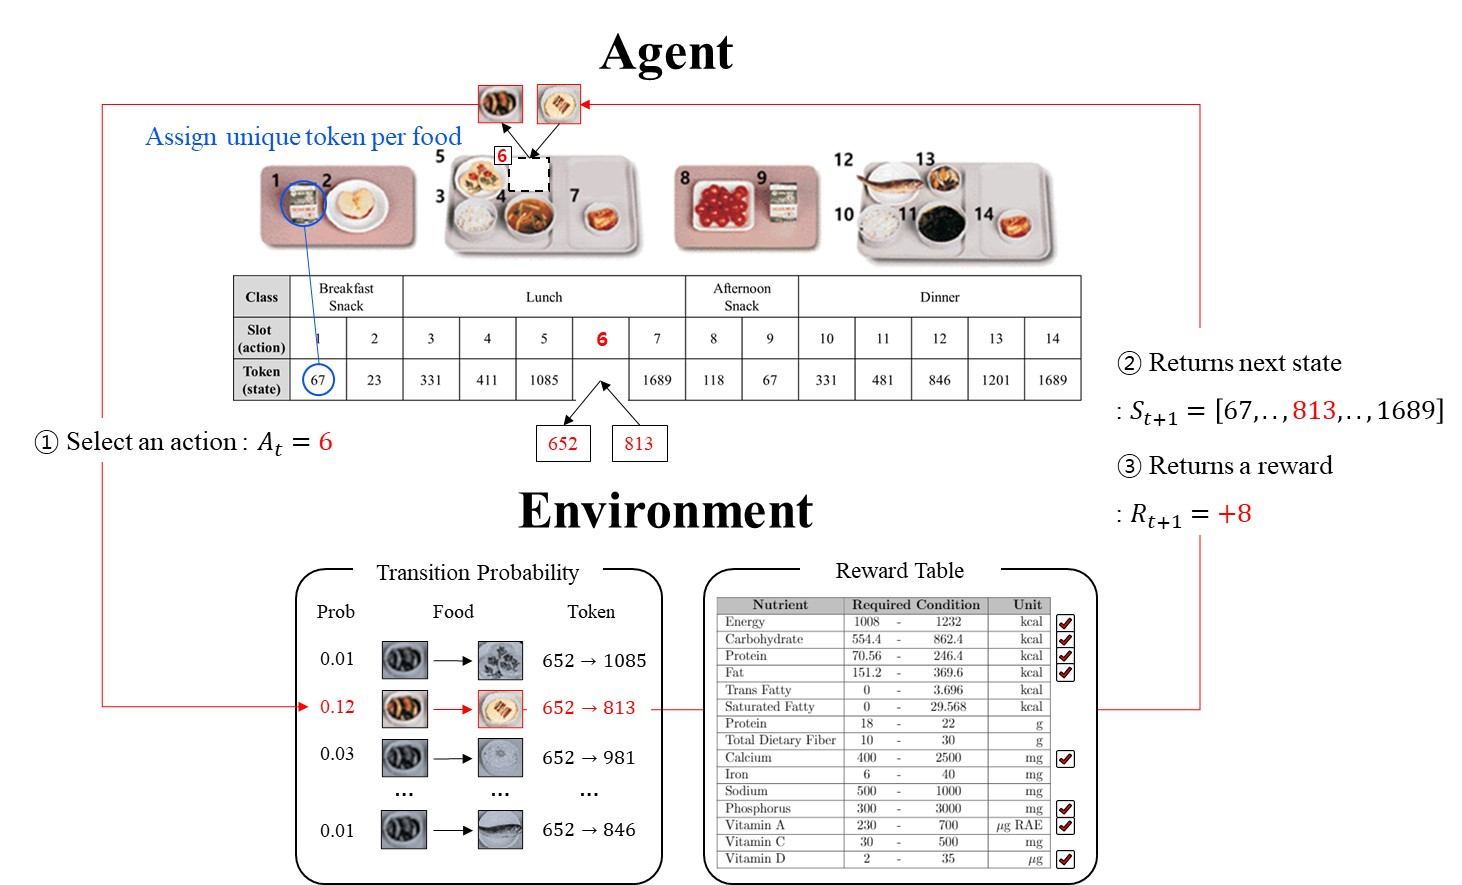
\includegraphics[width = 12cm, height = 7cm]{images/ad6.png}
    \caption{An overview of interaction between agent and environment for diet design}
    \label{fig:Overall Picture}
\end{figure}

In this work, we developed the RL-based AI solution that produces a daily diet plan (see Figure \ref{fig:Overall Picture}). Given that nutritionists sequentially adjust the foods while designing a diet, we modeled the diet design problem as the MDP. First, we defined the state to have an identical shape to a daily diet, similar to the real diet data in Table \ref{table: table2}. The state is as a vector of length 14, in which each element represents a food item in the diet. Each element is filled with a unique token randomly assigned to each food. In short, the state is the vectorized format of a diet.

Second, the agent selects one element (i.e., the agent makes an action) among the 14 elements of diet vector and removes the food in element. Then, the environment returns a new food to fill in the blank element, and the state with the new food becomes the next state. If the nutritional value of the next state is superior to that of the current state, the environment returns a reward to the agent. The nutrition quality of state is calculated by summing the individual nutritional values of each food items in the diet. We set the nutrient requirements of diet design based on the dietary reference intakes for Korean children aged 3-5 years. The number of nutrient requirements achieved at the given state was defined as the reward value. Table \ref{table: Nutrient Condition Table} shows the list of nutrients and their requirements to be achieved by the RL-based AI.

\begin{table}[ht]
\centering
\begin{tabular}{|l|ccc|r|}
\hline
\rowcolor[HTML]{C0C0C0} 
\multicolumn{1}{|c|}{\cellcolor[HTML]{C0C0C0}\textbf{Nutrient}} & \multicolumn{3}{c|}{\cellcolor[HTML]{C0C0C0}\textbf{Required Condition}} & \textbf{Unit} \\ \hline
Energy                                                          & 1008                 & -                & 1232                  & kcal          \\ \hline
Carbohydrate                                                    & 554.4                & -                & 862.4                 & kcal          \\ \hline
Protein                                                         & 70.56                & -                & 246.4                 & kcal          \\ \hline
Fat                                                             & 151.2                & -                & 369.6                 & kcal          \\ \hline
Trans Fatty                                                     & 0                    & -                & 3.696                 & kcal          \\ \hline
Saturated Fatty                                                 & 0                    & -                & 29.568                & kcal          \\ \hline
Protein                                                         & 18                   & -                & 22                    & g             \\ \hline
Total Dietary Fiber                                             & 10                   & -                & 30                    & g             \\ \hline
Calcium                                                         & 400                  & -                & 2500                  & mg            \\ \hline
Iron                                                            & 6                    & -                & 40                    & mg            \\ \hline
Sodium                                                          & 500                  & -                & 1000                  & mg            \\ \hline
Phosphorus                                                      & 300                  & -                & 3000                  & mg            \\ \hline
Vitamin A                                                       & 230                  & -                & 700                   & $\mu$g RAE         \\ \hline
Vitamin C                                                       & 30                   & -                & 500                   & mg            \\ \hline
Vitamin D                                                       & 2                    & -                & 35                    & $\mu$g            \\ \hline
\end{tabular}
\caption{A reward table of nutrients and their required conditions}
\label{table: Nutrient Condition Table}
\end{table}

Third, the agent is trained via interactions with the environment. The agent repeats the interactions to learn a policy that maximizes the total return. For training, we used the deep Q-learning \cite{watkins1989learning, mnih2013playing}. The update algorithm of Q-learning (equation \ref{eq:Algorithm of Q-learning}) aims to approximate the action-value function (equation \ref{eq:Q-function}) as accurately as possible. 

\begin{equation}
    Q(S_{t}, A_{t}) \leftarrow Q(S_{t}, A_{t}) + \alpha[R_{t+1} + \gamma \max_{a} Q(S_{t+1}, a) - Q(S_{t}, A_{t})]
\label{eq:Algorithm of Q-learning}
\end{equation}

\begin{equation}
    q_{\pi} \doteq \mathbb{E}_{\pi}[G_{t}|S_{t}=s, A_{t}=a] = \mathbb{E}_{\pi}[\sum_{k=0}^{\infty}\gamma^{k}R_{t+k+1}|S_{t}=s, A_{t}=a]
\label{eq:Q-function}
\end{equation}

This interaction is illustrated in Figure \ref{fig:Overall Picture}. If the agent judges arrival at a terminate state, the interaction ends. In this work, the terminate state is achievement of a recommended daily nutrient value that meets all the required conditions in Table \ref{table: Nutrient Condition Table}. At this time, the agent obtains a total return as maximized as possible. Therefore, RL-based AI always provides a nutritionally improved diet for children.

\listoffigures
\listoftables

\medskip
\bibliographystyle{vancouver}
\bibliography{sample}

\end{document}
